%!TEX program = xelatex
%!TEX root = geometria_analitica.tex
%%Usar makeindex -s indexstyle.ist arquivo.idx no terminal para gerar o {\'\i}ndice remissivo agrupado por inicial
%%Ap\'os executar pdflatex arquivo

\chapter{Quádricas} % (fold)
\label{cha:quadricas}

\section{Esfera} % (fold)
\label{sec:esfera}
\begin{definicao}
	\todo{Definição esfera}
\end{definicao}

\begin{figure}[!h]
	\centering
	\caption{Esfera: $x^2 + y^2 + z^2 = r^2$}
	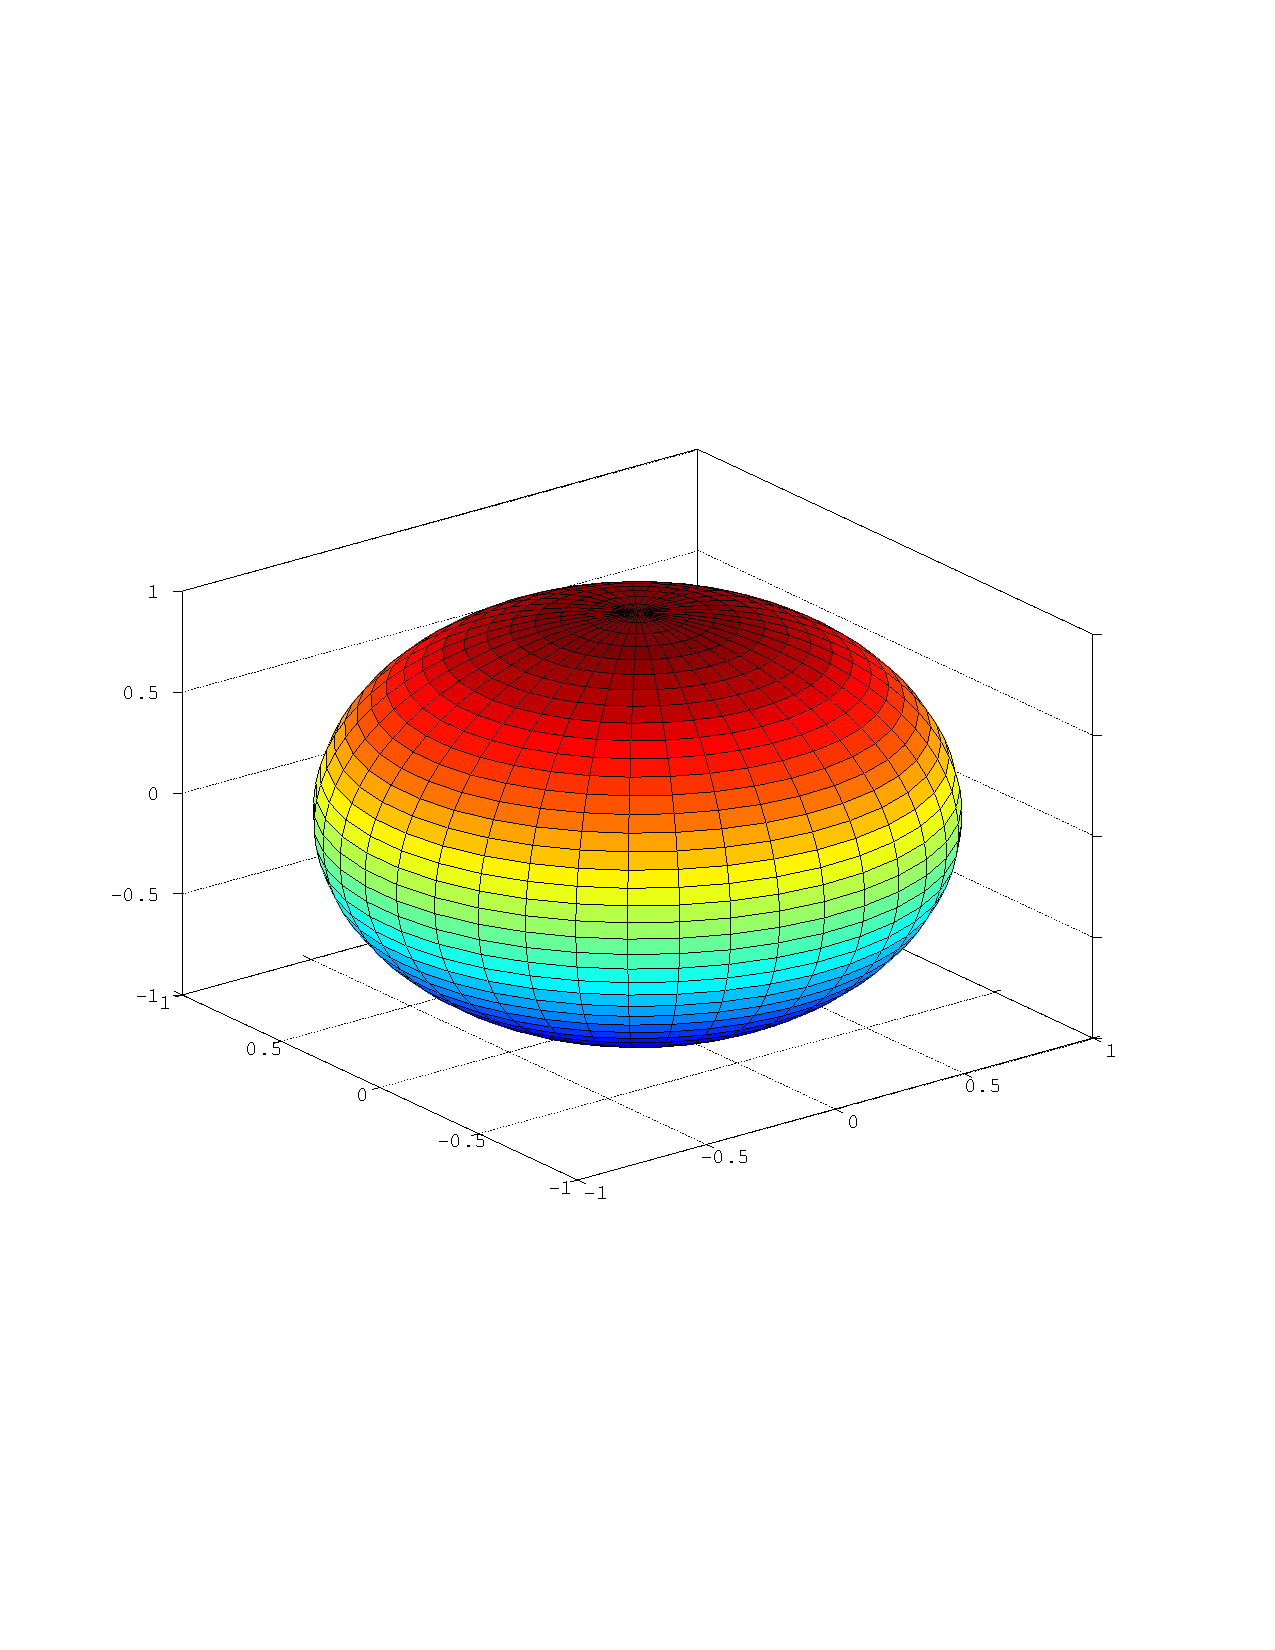
\includegraphics[scale=0.8]{quadricas/esfera.pdf}
	% \begin{pspicture}(-4,-2.25)(2,4.25)
	% \pstThreeDCoor[xMin=-3,yMax=3]
	% \pstThreeDSphere(0,0,0){2}
	% %\pstThreeDDot[dotstyle=x,linecolor=red,drawCoor=true](1,-1,2)
	% \end{pspicture}
\end{figure}

\begin{figure}[!h]
	\centering
	\caption{Contornos da esfera: $x^2 + y^2 + z^2 = r^2$}
	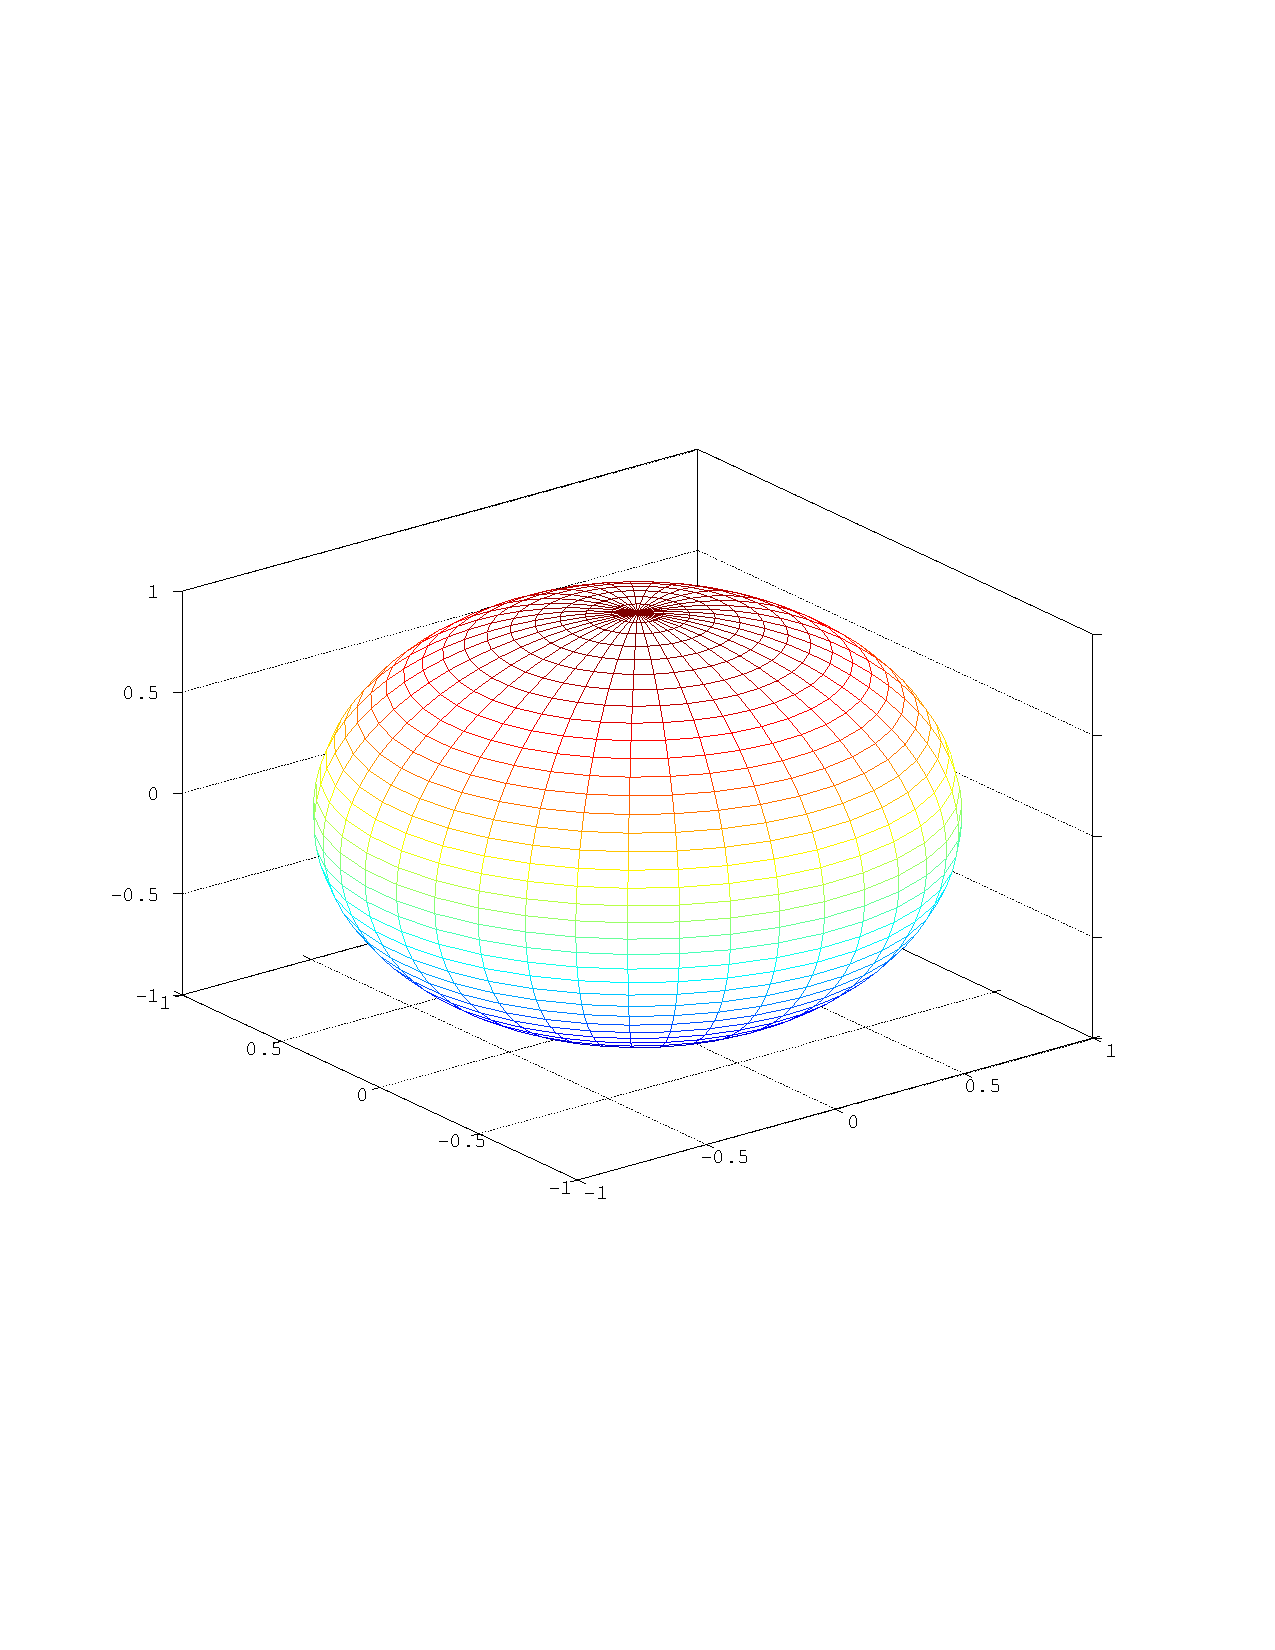
\includegraphics[scale=0.8]{quadricas/esfera-contornos.pdf}
	% \begin{pspicture}(-4,-2.25)(2,4.25)
	% \pstThreeDCoor[xMin=-3,yMax=3]
	% \pstThreeDSphere(0,0,0){2}
	% %\pstThreeDDot[dotstyle=x,linecolor=red,drawCoor=true](1,-1,2)
	% \end{pspicture}
\end{figure}
% section esfera (end)

\section{Elipsóide} % (fold)
\label{sec:elipsoide}
\begin{definicao}
	\todo{Definição esfera}
\end{definicao}
\begin{figure}[!h]
	\centering
	\caption{Elipsóide: $\dfrac{x^2}{a^2} + \dfrac{y^2}{b^2} + \dfrac{z^2}{c^2} = 1$}
	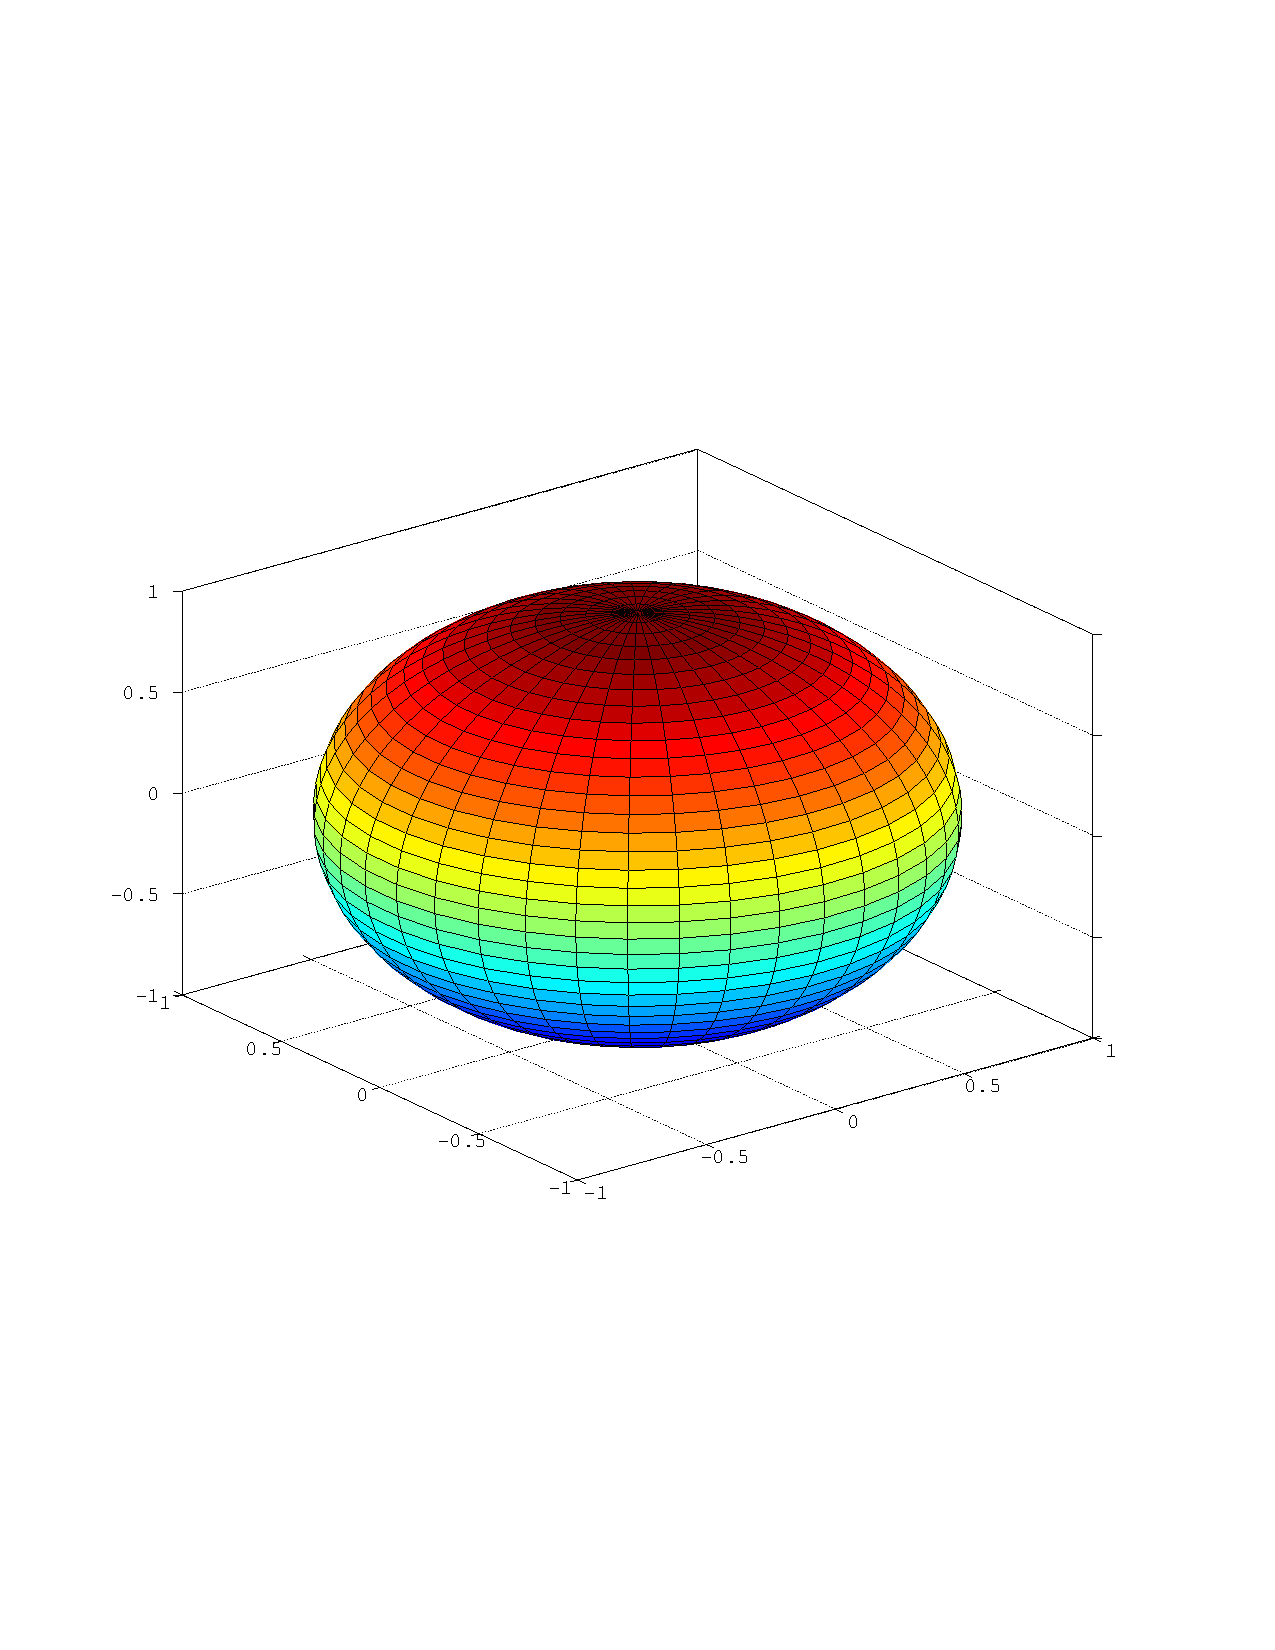
\includegraphics[scale=0.8]{quadricas/elipsoide.pdf}
		% \psset{unit=0.7}
	% \begin{pspicture*}(-4,-2)(4,3)
	% 	\psset[pst-solides3d]{viewpoint=40 40 20 rtp2xyz,Decran=20}
	% 	\psset{linewidth=0.5pt}
	% 	\defFunction[algebraic]{ellipsoid}(u,v){cos(u)*sin(v)}{2*sin(u)*sin(v)}{cos(v)}
	% 	\psSolid[object=surfaceparametree,
 %    		base=0 2 pi mul 0.001 2 pi mul,
 %    		hue=.3 0,incolor=yellow,
 %    		function=ellipsoid,
 %    		unit=3,ngrid=40]
	% 	\axesIIID(6,6,4)(8,8,5)
	% \end{pspicture*}
\end{figure}

\begin{figure}[!h]
	\centering
	\caption{Contornos do elipsóide $\dfrac{x^2}{a^2} + \dfrac{y^2}{b^2} + \dfrac{z^2}{c^2} = 1$}
	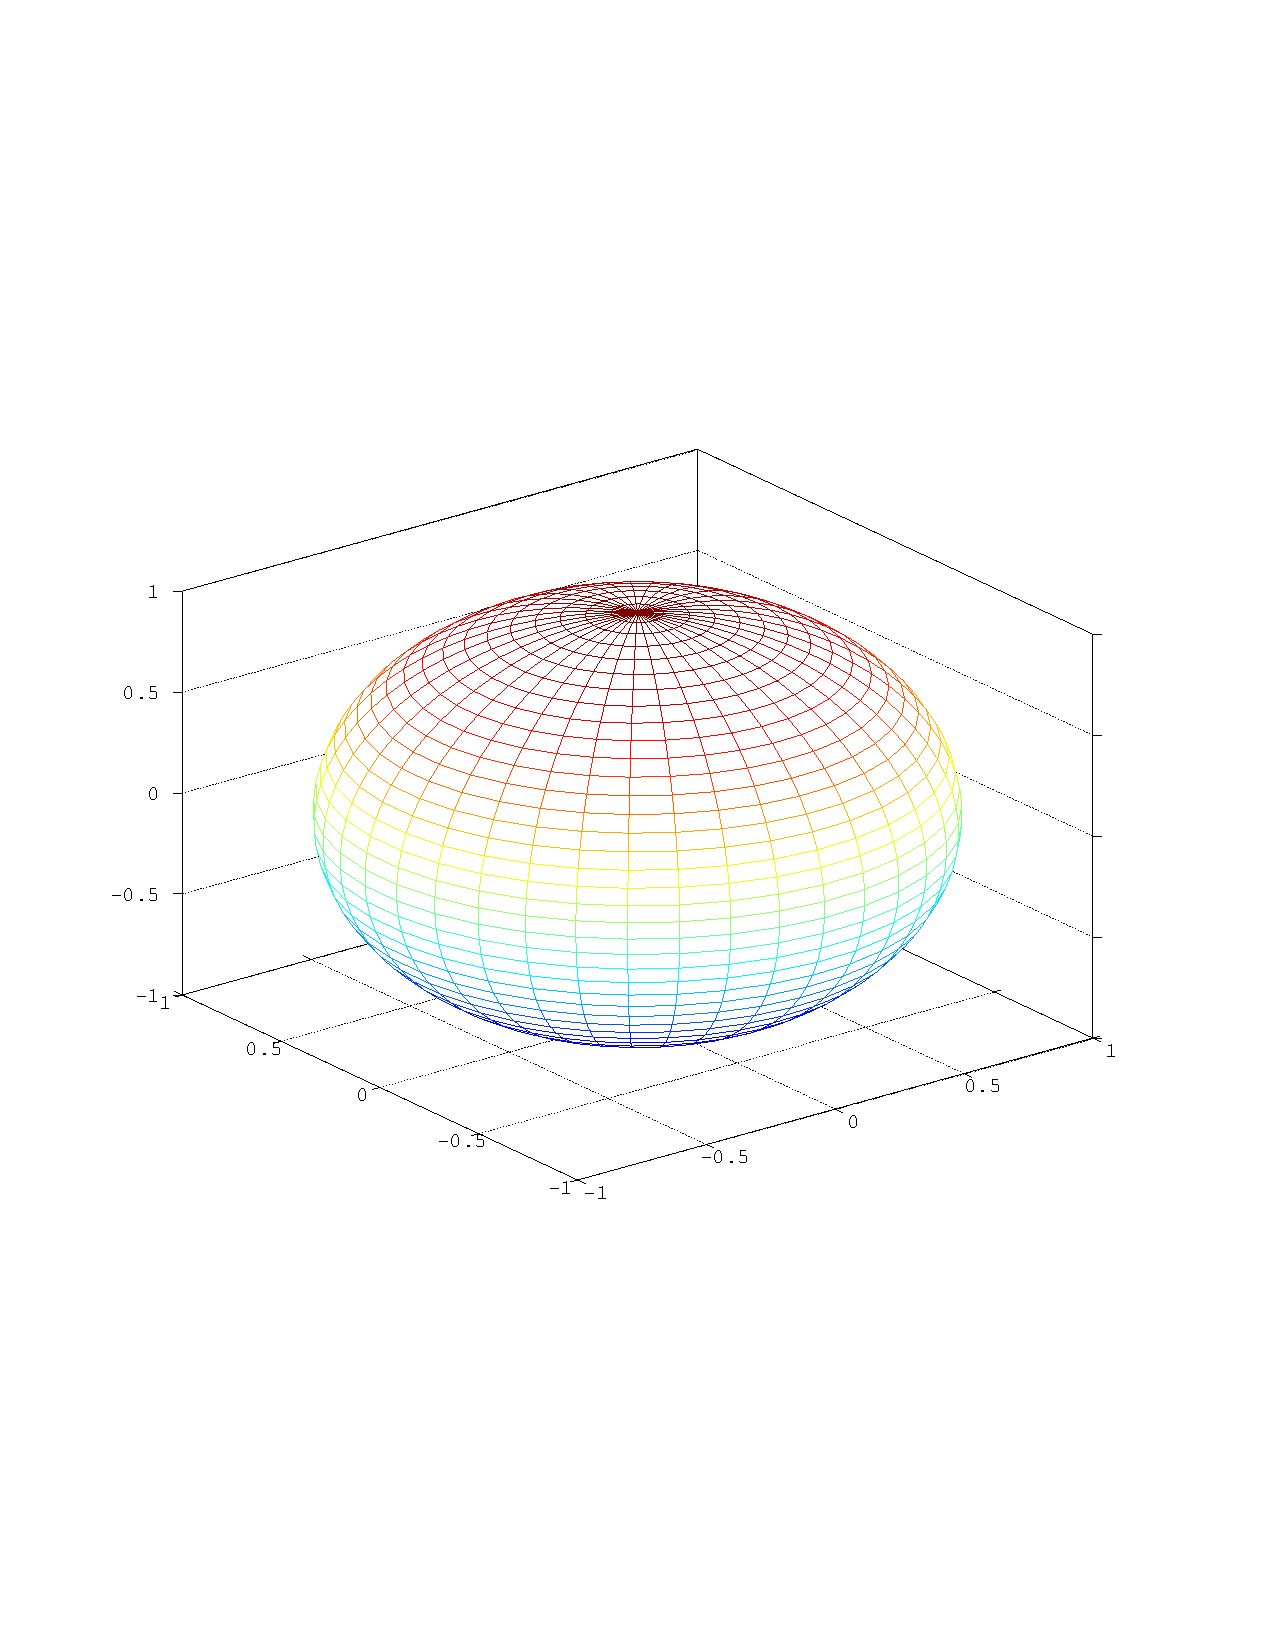
\includegraphics[scale=0.8]{quadricas/elipsoide-contornos.pdf}
	% \begin{pspicture}(-4,-2.25)(2,4.25)
	% \pstThreeDCoor[xMin=-3,yMax=3]
	% \pstThreeDSphere(0,0,0){2}
	% %\pstThreeDDot[dotstyle=x,linecolor=red,drawCoor=true](1,-1,2)
	% \end{pspicture}
\end{figure}

% section elipsoide (end)

\section{Parabolóide} % (fold)
\label{sec:paraboloide}
\begin{definicao}
	\todo[color=green]{Definição parabolóide}
\end{definicao}

\todo[color=red!50]{Equação parabolóide elíptico}
\begin{figure}[h]
	\centering
	\caption{Parabolóide Elíptico}
	% \psset{unit=0.5}
	% \begin{pspicture*}(-6,-2.7)(6,8.5)
	% 	\psset[pst-solides3d]{viewpoint=50 40 30 rtp2xyz,Decran=50}
	% 	\psset{ngrid=.25 .25,linewidth=0.5pt}
	% 	%superficie parametrica
	% 	\defFunction[algebraic]{Paraboloid}(u,v)
 %    		{u*sin(v)}{1.5*u*cos(v)}{0.5*u^2}
	% 	\psSolid[object=surfaceparametree,
 %    		base=0.001 pi 0.001 2 pi mul,
 %    		hue=0 .15,incolor=yellow,
 %    		function=Paraboloid]
	% 	\axesIIID(0,0,3)(5,5,8)
	% \end{pspicture*}
\end{figure}

\todo[color=blue!50]{Equação parabolóide hiperbólico}
\begin{figure}[h]
	\centering
	\caption{Parabolóide Hiperbólico}
	% \psset{unit=0.7}
	% \psset[pst-solides3d]{viewpoint=80 30 30 rtp2xyz,Decran=50}
 %    \psset{ngrid=.5 .5,linewidth=0.1pt}
 %    \begin{pspicture*}(-4,-3.5)(4,4)
 %       \psSurface[algebraic,hue=.3 0](-4,-4)(4,4){(y^2-x^2)/4}
 %       \axesIIID(0,3,0)(10,6,6)
 %    \end{pspicture*}
\end{figure}
% section paraboloide (end)

\section{Hiperbolóide} % (fold)
\label{sec:hiperboloide}
\begin{definicao}
	\todo[color=red!80]{Definição de hiperbolóide}
\end{definicao}

\todo[color=blue!50]{Equação do hiperbolóide de uma folha}
\begin{figure}[h]
	\centering
	\caption{Hiperbolóide de uma folha}
	% \psset{unit=0.7}
 %        \begin{pspicture*}(-4,-3)(4,3.8)
 %        \psset[pst-solides3d]{viewpoint=30 30 20 rtp2xyz,Decran=20}
 %        \psset{ngrid=.25 .25,linewidth=0.5pt}
 %        \defFunction[algebraic]{hyperboloidOne}(u,v){sqrt(1+u^2)*sin(v)}{sqrt(1+u^2)*cos(v)}{u}
 %        \psSolid[object=surfaceparametree, base=pi neg pi pi neg pi,hue=0 .3,incolor=yellow,function=hyperboloidOne]
 %        \axesIIID(1,1,1)(7,5,5)
 %    \end{pspicture*}
\end{figure}

\todo[color=blue!70]{Equação do hiperbolóide de duas folhas}
\begin{figure}[h]
	\centering
	\caption{Hiperbolóide duas folhas}
	% \psset{unit=0.6}
	% \begin{pspicture*}(-5.5,-4)(5.5,3.5)
	% 	\psset[pst-solides3d]{viewpoint=60 50 30 rtp2xyz,Decran=20}
	% 	\psset{algebraic,ngrid=.25 .25,linewidth=0.5pt}
	% 	%superficie parametrica
	% 	\defFunction{hyperboloidTwoN}(u,v){-2*u}{sqrt(u^2-1)*cos(v)}{sqrt(u^2-1)*sin(v)}
	% 	\psSolid[object=surfaceparametree,base=1.001 2 pi mul 0.01 2 pi mul,hue=.3 0,incolor=yellow,function=hyperboloidTwoN]
	% 	%superficie parametrica
	% 	\defFunction{hyperboloidTwo}(u,v){2*u}{sqrt(u^2-1)*sin(v)}{sqrt(u^2-1)*cos(v)}
	% 	\psSolid[object=surfaceparametree,base=1.001 2 pi mul 0.01 2 pi mul,hue=.3 0,incolor=yellow,function=hyperboloidTwo]
	% 	\axesIIID(-2,0,0)(16,8,8)
	% \end{pspicture*}
\end{figure}

% section hiperboloide (end)




\missingfigure{A lot of figures I have to make \ldots}


% \begin{figure}
	


% 	\parametricplotThreeD[plotstyle=curve,yPlotpoints=20](0,360)(0,1){t cos 2 mul u mul t sin u mul u dup mul 2 add}
% \end{figure}
% chapter quadricas (end)